%%
%% 5. Evaluation
%%
\section{Evaluation}

We evaluate FailureOps across four public QEC datasets and three intervention families. The main real-record evaluation uses the Google RL QEC detector-record release (40 conditions, 400,000 paired shots), with decoder-pathway intervention as the primary treatment. The pairing-necessity analysis uses bootstrap resampling over paired and unpaired estimators on the same conditions. The baseline comparison evaluates four conventional metrics---plain LFR, static detector burden, plain LFR delta, and unpaired bootstrap---against FailureOps paired sensitivity. The runtime-replay evaluation applies measured decoder service-time traces to a paired deadline intervention. The external and expanded evidence section covers the qec3v5 surface-code replication (§5.5), the Google RL QEC v2 496-condition expansion (§5.6), and the corpus-level decoder-prior study across 5,724 prior variants (§5.7). All statistical tests use exact McNemar tests over discordant rescued and induced transition counts, with scope-wise Holm correction applied at $\alpha = 0.05$ within each analysis scope.

\subsection{Main Real-Record Result}

The primary FailureOps intervention switches the decoder pathway from a SI1000-prior decoder to a frequency-calibrated-prior decoder, with both configurations operating on the same shot-level detector records. The SI1000 prior assumes all error mechanisms are equally likely (a uniform prior in error-mechanism space); the frequency-calibrated prior replaces this with a prior estimated from the observed detector-event frequencies on the same dataset. This intervention asks a concrete systems question: given the same detector records, does a data-driven prior outperform a uniform prior at rescuing logical failures?

The experiment spans 40 real-data conditions drawn from the Google RL QEC public dataset. The conditions form a full-factorial matrix of 2 control modes (reinforcement learning and traditional calibration) $\times$ 2 logical bases (X and Z) $\times$ 10 syndrome-extraction cycle settings (10 through 100, in steps of 10), all on surface-code memory experiments.

Table~\ref{tab:main_result} summarizes the main result. All 40 conditions exhibit a negative paired delta logical-failure rate, meaning the frequency-calibrated prior rescues more failures than it induces in every observed condition. The mean paired delta LFR is $-0.0195$, with the strongest single-condition effect reaching $-0.0369$ and the weakest at $-0.0019$. Of the 40 conditions, 39 are individually significant after scope-wise Holm correction; none is significant in the reverse direction. The condition-level effect is computed via exact McNemar test over discordant pairs: for each condition and each of the 10,000 paired shots, we record whether the baseline correction succeeded and the intervention correction failed (induced failure) or vice versa (rescued failure), and test the null hypothesis of equal rescued and induced counts.

The significance framework applies Holm correction within the analysis scope \texttt{real\_decoder\_pathway}, which contains exactly these 40 conditions. This means the family-wise error rate is controlled at 0.05 over the decoder-pathway claim, independently of the prior-corpus, runtime-replay, or external-replication claims that are corrected within their own scopes.

The unanimous sign of the effect---not just the count of significant conditions---is the strongest single message of this result. Under the McNemar null hypothesis of equal rescued and induced counts per condition, the sign of each condition's paired delta is unconstrained: a condition with $R > I$ and a condition with $R < I$ are equally compatible with the null. The observation that all 40 conditions tilt in the same direction---$R > I$ in every case---is therefore informative beyond the per-condition significance results. This pattern is what we would expect if the frequency-calibrated prior systematically improves correction quality on these real detector records, and FailureOps paired counterfactual measurement is sensitive enough to capture it.

\begin{figure}[t]
\centering

\includegraphics[width=\columnwidth]{figures/p10_eurosys_main_evidence.png}
\caption{Per-condition paired delta LFR for the main decoder-pathway intervention across 40 real-data conditions.}
\label{fig:main_result}
\end{figure}

\begin{table}[t]
\centering
\caption{Summary of the main decoder-pathway intervention on 40 Google RL QEC real-data conditions.}
\label{tab:main_result}
\begin{tabular}{lr}
\toprule
Metric & Value \\
\midrule
Total conditions & 40 \\
Net-rescuing conditions & 40 \\
Holm-significant conditions ($\alpha = 0.05$) & 39 \\
Mean paired delta LFR & $-0.0195$ \\
Min paired delta LFR & $-0.0369$ \\
Max paired delta LFR & $-0.0019$ \\
Total paired shots & 400,000 \\
\bottomrule
\end{tabular}
\end{table}

\subsection{Why Pairing Is Necessary}

The paired design is not a statistical preference; it is a measurement requirement. Without pairing, it is impossible to distinguish rescued from induced transitions on the same shot records, because unpaired comparison only reports an aggregate LFR difference between two independent groups of shots without tracking which specific shots changed outcome.

We quantify the cost of discarding pairing through bootstrap resampling. For each of the 40 original real-data conditions, we compute the paired bootstrap standard deviation of the delta LFR (preserving shot-level pairing across 300 resamples) and the unpaired bootstrap standard deviation (independently resampling baseline and intervened outcomes). Table~\ref{tab:pairing} reports the results. Across all 40 conditions, the mean ratio of unpaired to paired bootstrap standard deviation is 1.75, with a minimum of 1.52 and a maximum of 2.05. In every single condition, the unpaired estimator exhibits higher standard deviation than its paired counterpart.

We repeat the same analysis on the expanded 496-condition Google RL QEC v2 corpus. The mean ratio is 1.78, with a wider range of 1.06 to 3.09. Again, no condition shows a ratio below 1.0. The worst-case condition on the v2 corpus exhibits an unpaired standard deviation more than three times larger than the paired estimate.

The practical consequence is that an unpaired estimator would require between 2.3$\times$ and 9.6$\times$ more samples to achieve the same confidence-interval width as the paired estimator, assuming standard asymptotic scaling. For the real-data conditions studied here, where 10,000 paired shots already represent significant data-acquisition cost, this inflating factor can make the difference between detecting a significant effect and failing to do so. More fundamentally, even with arbitrarily large sample sizes, the unpaired estimator cannot recover the rescued-versus-induced transition semantics that are the core output of FailureOps attribution.

\begin{figure}[t]
\centering
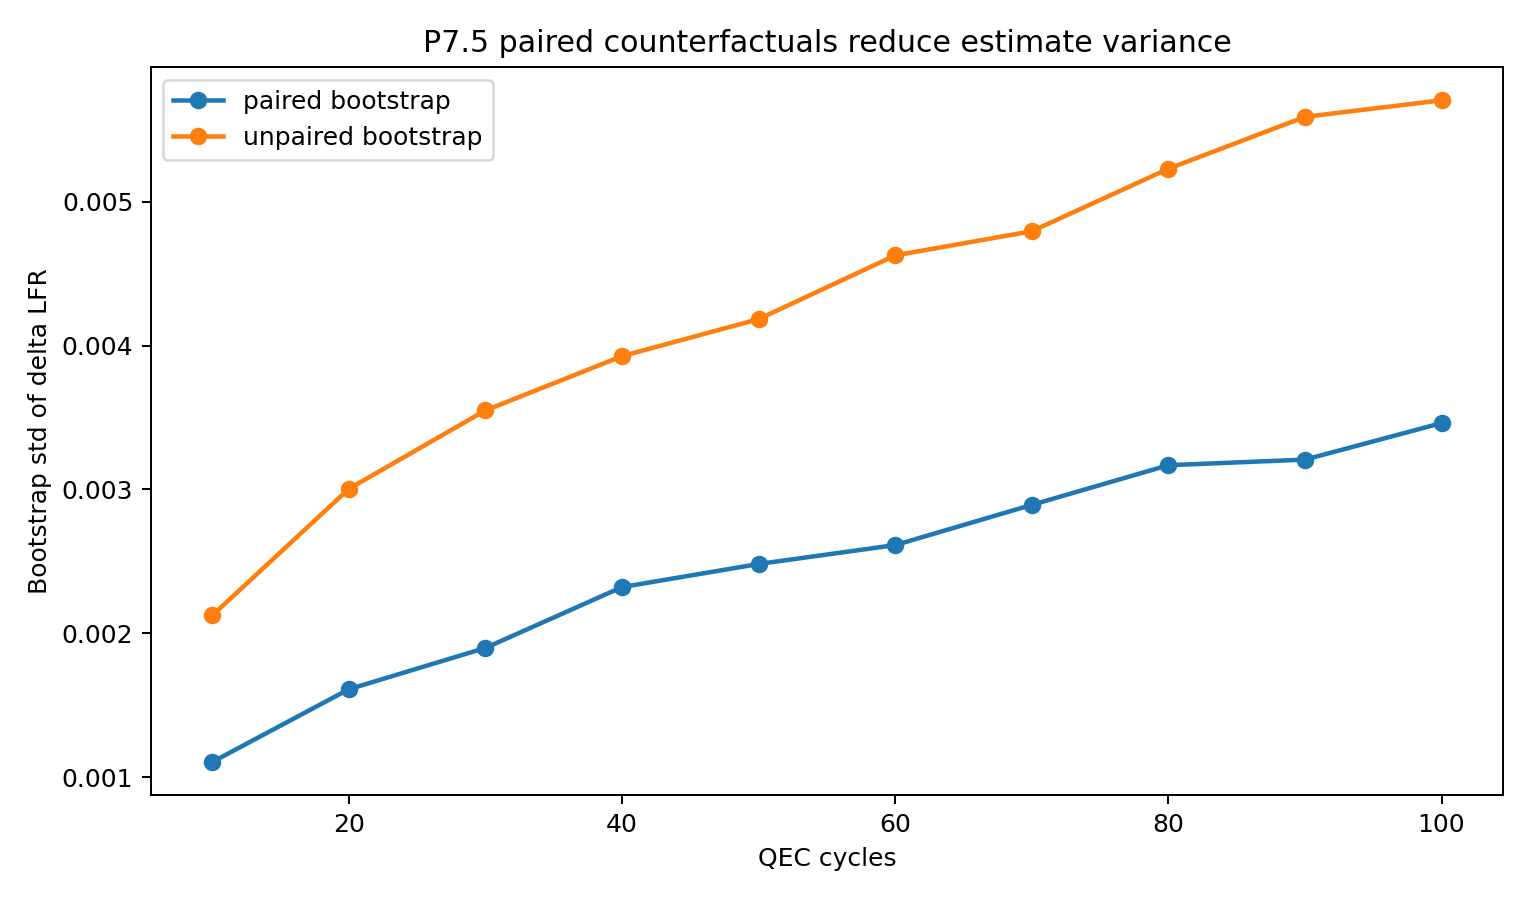
\includegraphics[width=\columnwidth]{figures/p7_5_paired_vs_unpaired_variance.png}
\caption{Paired versus unpaired bootstrap standard deviation across the 40 original real-data conditions. Every condition falls above the 1:1 line, indicating higher unpaired variance.}
\label{fig:pairing}
\end{figure}

\begin{table}[t]
\centering
\caption{Paired versus unpaired bootstrap standard deviation ratios.}
\label{tab:pairing}
\begin{tabular}{lrrr}
\toprule
Corpus & Conditions & Mean ratio & Range \\
\midrule
Original (40 conditions) & 40 & 1.75 & 1.52--2.05 \\
V2 expanded (496 conditions) & 496 & 1.78 & 1.06--3.09 \\
\bottomrule
\end{tabular}
\end{table}

\subsection{Baseline Comparison}

We compare FailureOps paired sensitivity against five conventional metrics: plain baseline LFR, static detector burden, plain LFR delta (intervened minus baseline, aggregated), an unpaired bootstrap estimator, and a ranking-by-LFR-delta approach. The question is not whether these baselines are accurate predictors of LFR---several of them correlate strongly with condition difficulty. The question is whether they can substitute for intervention attribution.

Table~\ref{tab:baselines} summarizes the comparison. Plain baseline LFR achieves a Spearman rank correlation of 0.963 with FailureOps paired sensitivity, and static detector burden achieves 0.950. These high correlations indicate that difficult conditions---those with higher baseline LFR or higher detector event counts---also tend to exhibit larger intervention effects. However, the top-3 overlap with the FailureOps sensitivity ranking is only 0.333 for static burden and 0.667 for plain LFR, meaning the most intervention-sensitive conditions are not consistently the conditions flagged by these baselines.

More critically, neither baseline provides rescued or induced transition counts. Consider the most intervention-sensitive condition in the FailureOps ranking (surface\_code\_traditional\_calibration, X basis, 90 cycles): it exhibits a paired delta of $-0.037$ with a large rescued-to-induced imbalance, yet it is not the top-ranked condition by baseline LFR (which instead flags the 100-cycle X-basis condition) or by static detector burden (which flags a Z-basis condition at 100 cycles). The baselines identify difficult conditions but cannot explain why this particular condition is the most sensitive to a decoder-prior change, nor can they decompose its 10,000 paired outcomes into rescued, induced, and unchanged transitions. Plain LFR reports the aggregate failure rate under a single configuration; it does not by itself identify which controllable factor changes failure behavior. Plain LFR delta, when computed over paired records as in our setup, numerically agrees with the paired delta LFR (Spearman 0.9998), but this agreement is an artifact of pairing: without the paired framework, an unpaired LFR delta would conflate rescued and induced transitions into a single aggregate difference, losing the transition semantics that distinguish FailureOps attribution from aggregate comparison.

The unpaired bootstrap estimator, as shown in the previous subsection, carries 1.5--3.1$\times$ higher standard deviation than the paired estimator and cannot recover per-shot transition labels on its own.

\begin{table}[t]
\centering
\caption{Comparison of FailureOps paired sensitivity against conventional metrics.}
\label{tab:baselines}
\begin{tabular}{lcc}
\toprule
Metric & Spearman $\rho$ & Top-3 overlap \\
\midrule
Plain baseline LFR & 0.963 & 0.667 \\
Static detector burden & 0.950 & 0.333 \\
Plain LFR delta (paired) & 0.999 & 0.667 \\
\midrule
FailureOps paired sensitivity & 1.000 & 1.000 \\
\bottomrule
\end{tabular}
\end{table}

The takeaway is not that the baselines are weak---several of them correlate strongly with condition difficulty---but that they answer a different question. Ranking conditions by difficulty is not the same as attributing failure behavior to a specific controllable intervention. The information that FailureOps adds is not a better correlation coefficient; it is the rescued and induced transition semantics that connect interventions to logical outcomes on the same physical shots.

\subsection{Runtime Replay Closure}

The fourth intervention family applies a measured-runtime deadline to decoder corrections. We use decoder service-time measurements collected on the same real detector records (mean service time 4.65\,$\mu$s, p95 5.64\,$\mu$s) and apply a paired deadline intervention: if the measured service time for a shot exceeds a deadline budget, the correction is treated as late and dropped to a default no-flip correction. We evaluate five deadline budgets in $\{4, 5, 6, 7, 8\}$\,$\mu$s on 10,000 paired shots.

Table~\ref{tab:runtime} reports the results. The effect is sharply thresholded. A 4\,$\mu$s deadline causes a 93.6\% miss rate---93.6\% of corrections arrive too late---and induces a paired delta LFR of $+0.307$, with 185 rescued and 3,257 induced failures. This is the only deadline condition that is individually Holm-significant. At 5\,$\mu$s, the miss rate drops to 19.4\% and the paired delta LFR to $+0.064$ (32 rescued, 668 induced). At 6\,$\mu$s, only 1.3\% of corrections miss the deadline, and the delta LFR is negligible at $+0.004$. At 7\,$\mu$s and above, the miss rate reaches zero and no logical-failure effect remains.

\begin{table}[t]
\centering
\caption{Runtime deadline intervention results. Mean measured service time is 4.65\,$\mu$s, p95 is 5.64\,$\mu$s.}
\label{tab:runtime}
\begin{tabular}{lrrrrr}
\toprule
Deadline & Miss rate & Baseline LFR & Intervened LFR & $\Delta$LFR & Holm sig. \\
\midrule
4\,$\mu$s & 0.936 & 0.040 & 0.347 & $+0.307$ & Yes \\
5\,$\mu$s & 0.194 & 0.040 & 0.103 & $+0.064$ & No \\
6\,$\mu$s & 0.013 & 0.040 & 0.044 & $+0.004$ & No \\
7\,$\mu$s & 0.000 & 0.040 & 0.040 & 0.000 & No \\
8\,$\mu$s & 0.000 & 0.040 & 0.040 & 0.000 & No \\
\bottomrule
\end{tabular}
\end{table}

The threshold behavior---the sharp transition from a large effect at 4\,$\mu$s to near-zero effect at 6\,$\mu$s---is a direct consequence of the decoder service-time distribution. The mean service time (4.65\,$\mu$s) lies between the 4\,$\mu$s and 5\,$\mu$s budgets, and the p95 (5.64\,$\mu$s) sits between the 5\,$\mu$s and 6\,$\mu$s budgets. A system operator who must set a decoder deadline based on measured service time faces a genuine engineering tradeoff: a 4\,$\mu$s budget guarantees fast cycle times but induces substantial logical failures; a 6\,$\mu$s budget eliminates the induced failures but requires longer cycle times; the 5\,$\mu$s budget represents a gray zone.

We call this measured-runtime replay closure, not live control-stack timing attribution. The service-time measurements are collected on real detector records, but they are not obtained from an actual quantum control stack with hardware feedback latency, production queueing, or real-time scheduling. The replay demonstrates that decoder service time can be turned into a paired intervention whose effect on logical outcomes can be quantified on the same shot records. Closing this loop with live-hardware timing traces remains future work.

\begin{figure}[t]
\centering
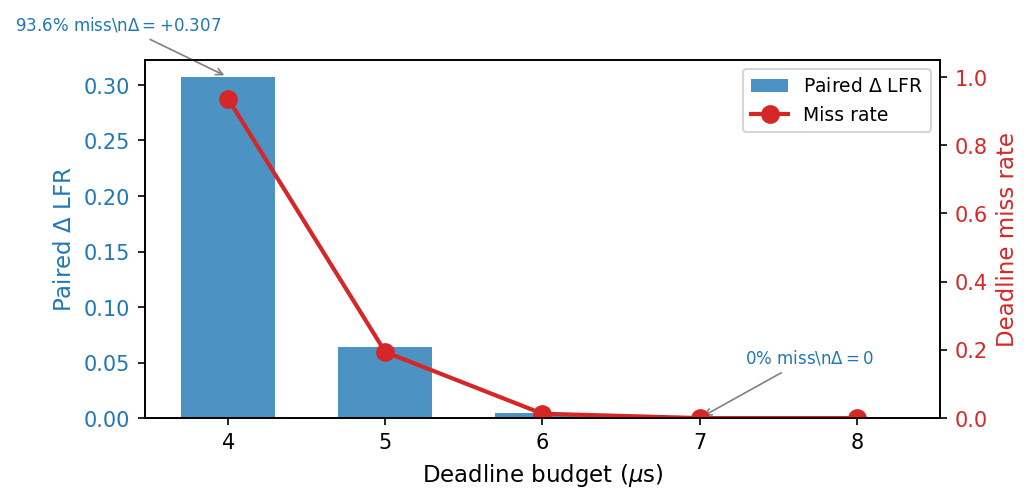
\includegraphics[width=\columnwidth]{figures/p10_runtime_deadline_threshold.png}
\caption{Paired delta LFR (bars) and deadline miss rate (line) as a function of decoder deadline budget. A sharp threshold appears between 4\,$\mu$s and 6\,$\mu$s, corresponding to the region around the measured mean service time of 4.65\,$\mu$s.}
\label{fig:runtime}
\end{figure}

\subsection{External Replication on qec3v5}
\label{sec:qec3v5}

The Google qec3v5 2022 surface-code scaling dataset provides an independent test of the decoder-pathway sensitivity result. The qec3v5 dataset uses a different code family (rotated surface code, distance 5), a different decoder baseline (PyMatching), and a different experimental setup (syndrome sampling at 13 cycle depths from $r = 1$ to $r = 25$). We apply the same paired counterfactual design, switching from PyMatching to a correlated-matching decoder on 10,000 paired shots per condition.

\begin{figure}[t]
\centering
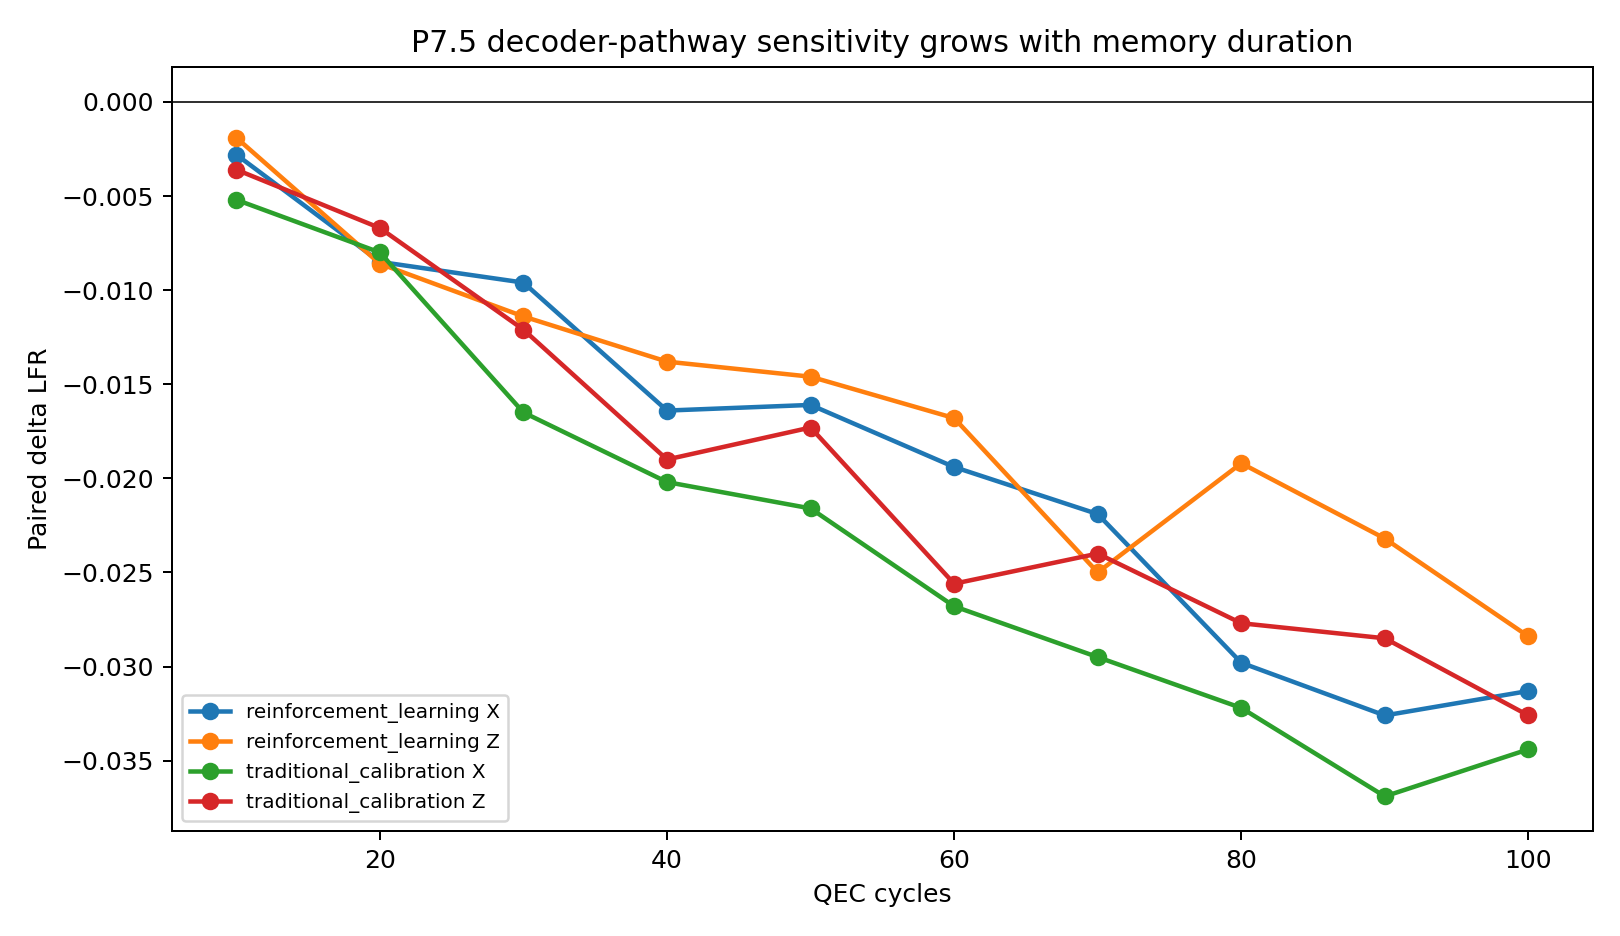
\includegraphics[width=\columnwidth]{figures/p7_5_decoder_effect_by_cycles.png}
\caption{Paired delta LFR by cycle depth on the qec3v5 surface-code dataset. The effect strengthens monotonically with memory duration and is consistent across X and Z bases.}
\label{fig:qec3v5}
\end{figure}

Of the 26 conditions (13 X-basis, 13 Z-basis), 23 are individually significant after scope-wise Holm correction. The mean paired delta LFR is $-0.0279$ for X-basis conditions and $-0.0268$ for Z-basis conditions. The three non-significant conditions are the shortest-cycle conditions ($r = 1$ for X and Z, where the baseline LFR is below 0.01), which is consistent with the observation that intervention sensitivity grows with memory duration. Table~\ref{tab:qec3v5} summarizes the cycle-level breakdown: the effect strengthens monotonically from $r = 1$ ($\Delta = -0.0001$, not significant) to $r = 11$ ($\Delta = -0.036$) and remains negative through all higher cycle settings. This external replication, on a different dataset with a different decoder baseline, supports the claim that decoder-pathway sensitivity is not an artifact of a particular code, decoder, or experiment design.

\begin{table}[t]
\centering
\caption{qec3v5 external replication: paired delta LFR by cycle depth.}
\label{tab:qec3v5}
\begin{tabular}{lrrr}
\toprule
Cycles & Conditions & Mean $\Delta$LFR & Holm sig. \\
\midrule
1 & 2 & $-0.0001$ & 0/2 \\
3--9 & 8 & $-0.0219$ & 8/8 \\
11--25 & 16 & $-0.0333$ & 15/16 \\
\midrule
All & 26 & $-0.0274$ & 23/26 \\
\bottomrule
\end{tabular}
\end{table}

\subsection{Expanded Same-Family Stability on Google RL QEC v2}

The Google RL QEC v2 corpus expands the original 40-condition matrix to 496 conditions with 4.96 million paired shots. The expansion adds three dimensions: a second code family (color-code memory, 48 conditions), a second control mode (traditional\_calibration\_and\_rl\_fine\_tuning, which doubles the control-mode dimension from 1 to 2), and additional cycle settings up to 150 rounds. The overall mean paired delta LFR is $-0.014$, and 461 of 496 conditions (92.9\%) are net-rescuing. After scope-wise Holm correction, 273 conditions are individually significant.

Table~\ref{tab:v2_subgroups} breaks down the effect by subgroup. The mean paired delta is negative in every observed subgroup, with no reversal. Color-code memory conditions show a slightly stronger mean effect ($-0.017$) than surface-code memory ($-0.013$). Z-basis conditions ($-0.016$) show a moderately larger effect than X-basis ($-0.011$). The two control modes---traditional\_calibration and traditional\_calibration\_and\_rl\_fine\_tuning---produce nearly identical mean deltas ($-0.014$ and $-0.013$ respectively). The subgroup stability reinforces the main result: the paired sensitivity signal is not confined to a particular code, basis, or calibration mode but appears broadly across the expanded public real-record corpus.

\begin{figure}[t]
\centering
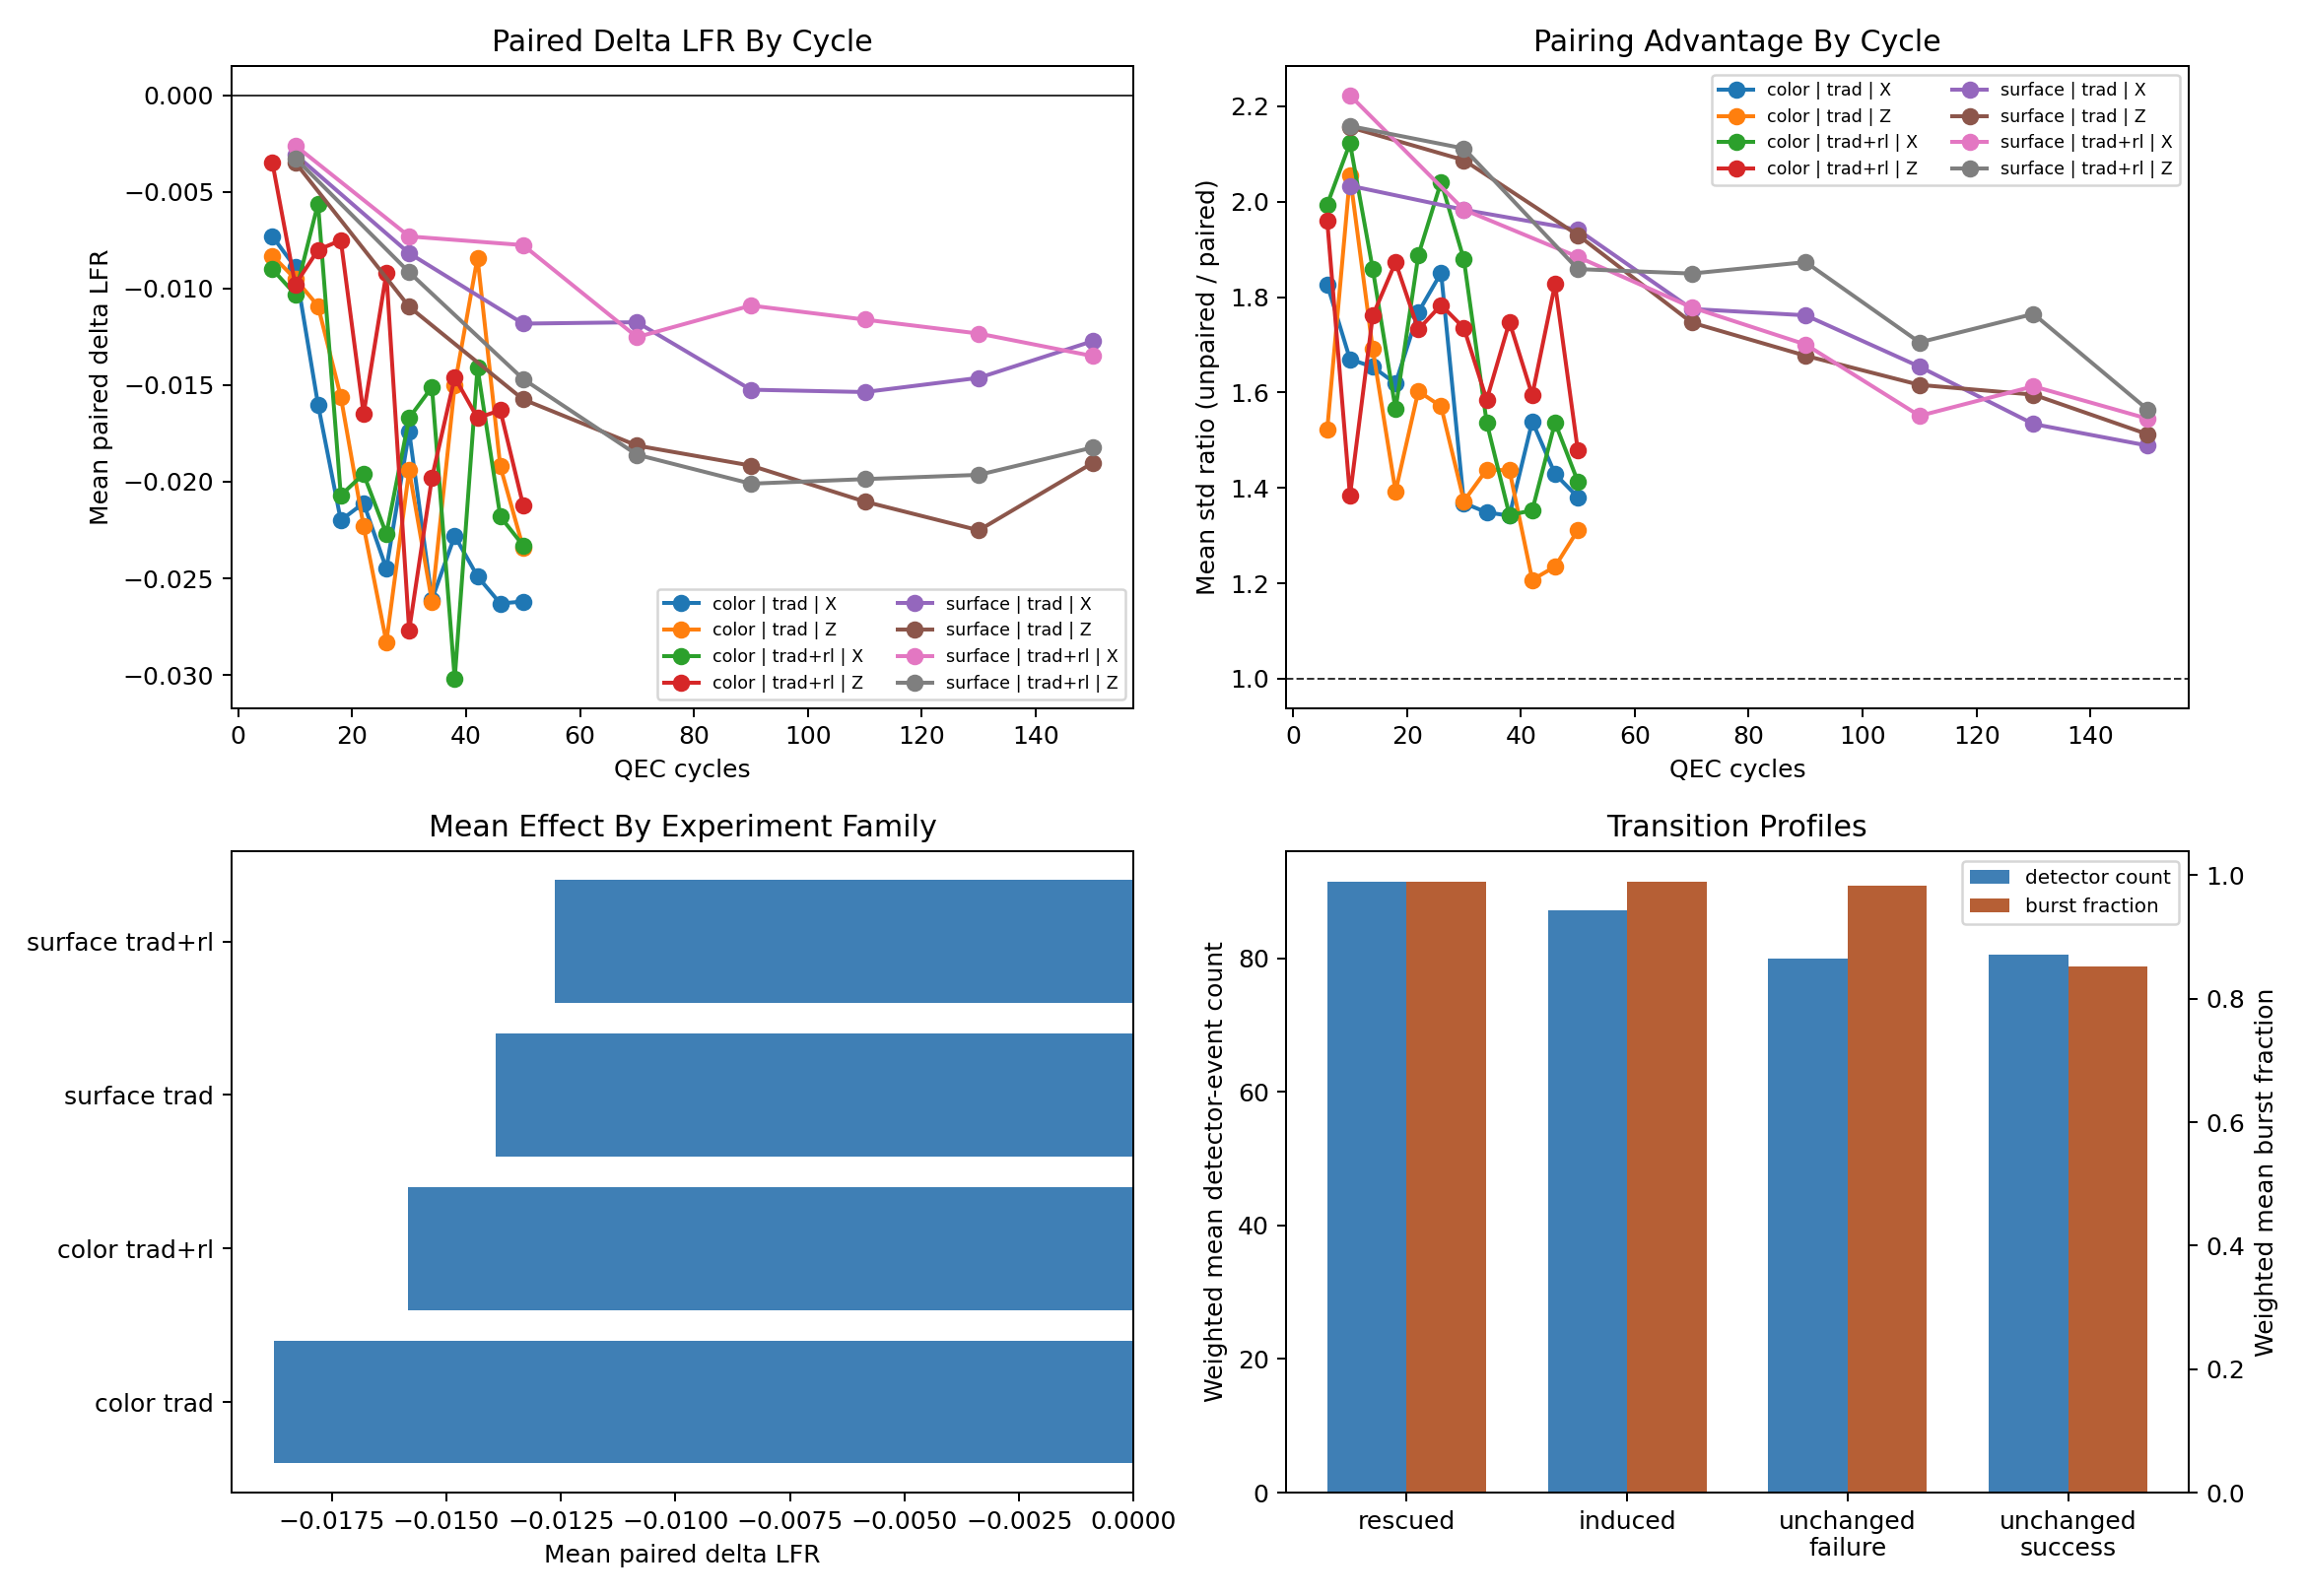
\includegraphics[width=\columnwidth]{figures/p10_google_rl_qec_v2_evidence.png}
\caption{Expanded Google RL QEC v2 evidence: per-condition paired delta LFR across 496 conditions (top left), paired-vs-unpaired variance ratio (top right), subgroup aggregation (bottom left), and rescued/induced transition profiles (bottom right).}
\label{fig:v2}
\end{figure}

\begin{table}[t]
\centering
\caption{Google RL QEC v2 subgroup breakdown. All subgroups show negative mean paired delta LFR.}
\label{tab:v2_subgroups}
\begin{tabular}{lrr}
\toprule
Subgroup & Conditions & Mean $\Delta$LFR \\
\midrule
Surface code memory & 448 & $-0.013$ \\
Color code memory & 48 & $-0.017$ \\
\addlinespace
Traditional calibration & 248 & $-0.014$ \\
RL fine tuning & 248 & $-0.013$ \\
\addlinespace
X basis & 248 & $-0.011$ \\
Z basis & 248 & $-0.016$ \\
\midrule
All v2 conditions & 496 & $-0.014$ \\
\bottomrule
\end{tabular}
\end{table}

This v2 expansion broadens the Google public corpus substantially, but it remains same-family evidence: both the original and v2 datasets come from the Google RL QEC release. We treat this as expanded stability evidence rather than independent cross-platform replication.

\subsection{Corpus-Level Decoder-Prior Study}

Scaling further, we evaluate whether the decoder-prior sensitivity observed on the SI1000-to-frequency-calibrated switch generalizes across prior variants within a fixed decoder family. The decoder-prior corpus study intervenes on three prior families---dem\_correlations, dem\_rl\_isolated\_correlated\_matching, and dem\_rl\_shared\_correlated\_matching---each compared against a common dem\_simple baseline, covering 1,908 real-data conditions per family. The total corpus spans 5,724 prior variants with 19.08 million paired shots.

Of the 5,724 variants, 4,879 (85.2\%) yield bootstrap confidence intervals that exclude zero. The mean paired delta LFR is negative in all three prior families: $-0.0133$ (dem\_correlations), $-0.0212$ (dem\_rl\_isolated), and $-0.0180$ (dem\_rl\_shared). The negative-delta fraction reaches 0.983, 0.997, and 0.960 respectively. The strongest single prior variant achieves a paired delta of $-0.0494$.

This result serves two purposes in the FailureOps evaluation. First, it demonstrates scale: the paired counterfactual pipeline can be applied to thousands of intervention variants without modification, producing comparable sensitivity metrics across an intervention design space. Second, it shows that decoder-prior sensitivity is not a single binary switch but a spectrum: different prior designs produce different effect magnitudes while preserving the negative sign. For a systems audience, this is analogous to a parameter-sensitivity study over a scheduler or allocator design space---the intervention becomes a tunable family rather than a binary treatment.

\begin{figure}[t]
\centering
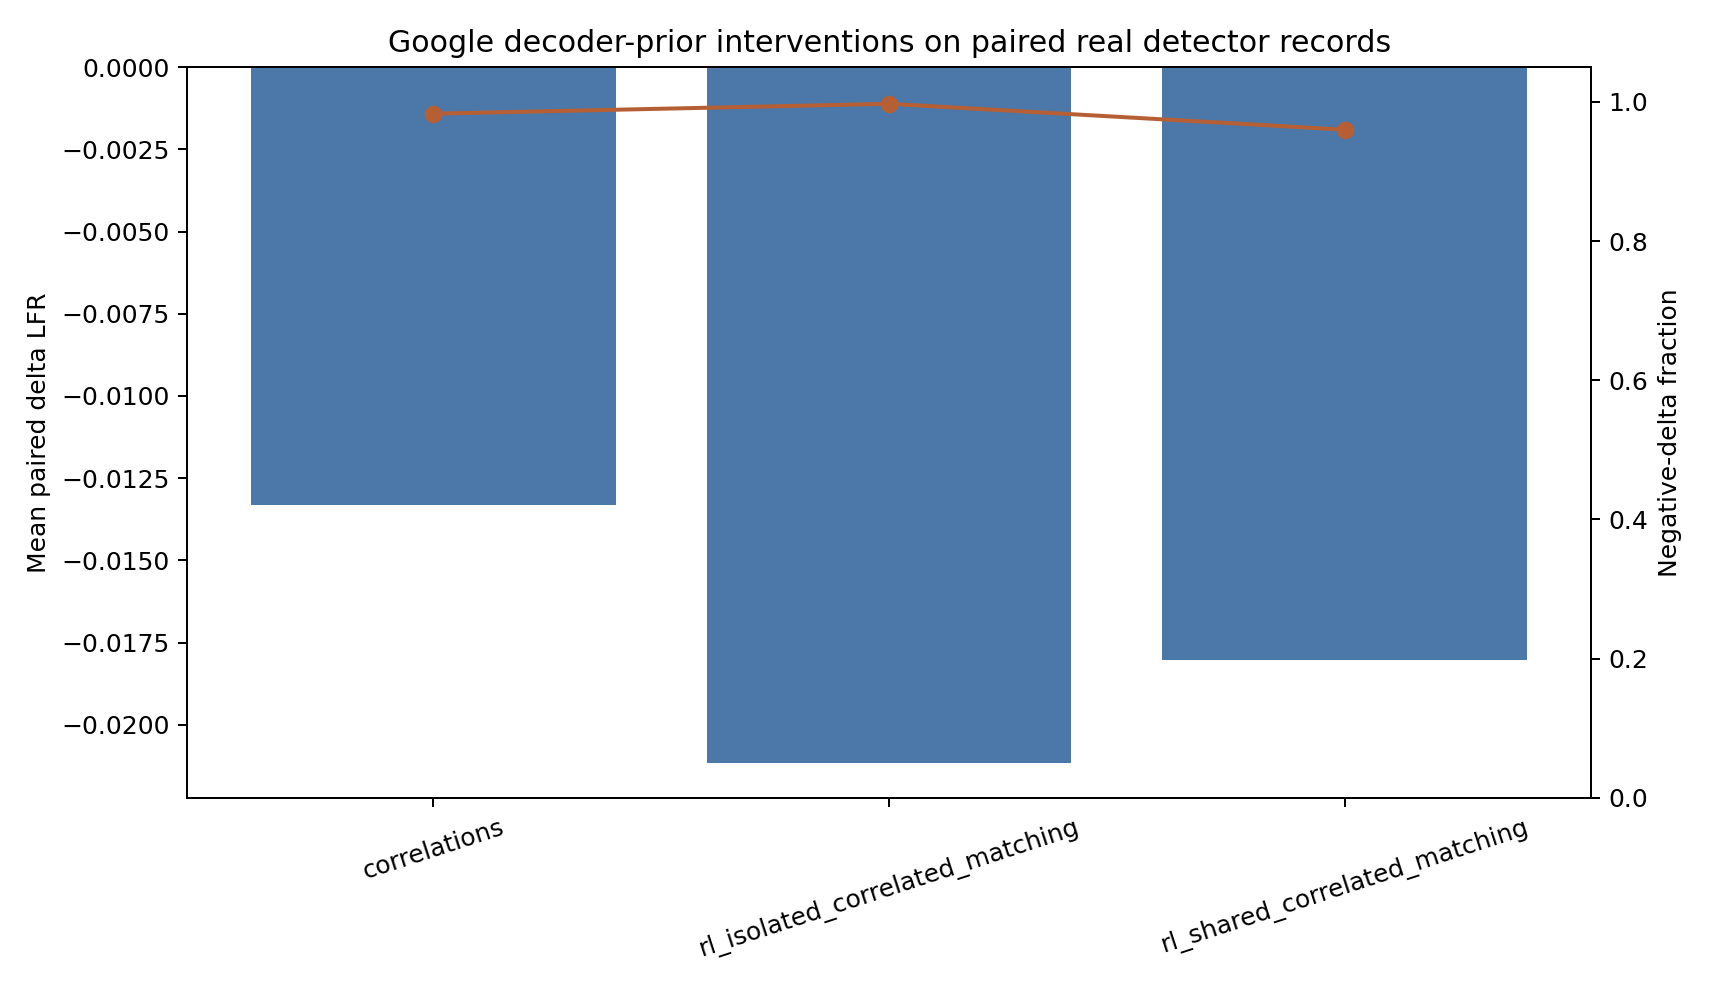
\includegraphics[width=\columnwidth]{figures/p10_google_decoder_priors_prior_effects.png}
\caption{Distribution of paired delta LFR across 5,724 decoder-prior variants. The histogram peak lies in the negative region, confirming that most alternative prior configurations rescue more failures than the baseline SI1000 prior.}
\label{fig:prior_corpus}
\end{figure}

\subsection{Characterizing Rescued Shots}
\label{sec:rescued_shot_analysis}

The preceding subsections establish that the frequency-calibrated prior rescues more failures than it induces across all 40 conditions. This section goes one step further by interrogating \emph{which kinds of detector-event patterns} distinguish rescued shots from unchanged-failure shots. The goal is not to propose a new error model, but to connect the observed intervention effect to the physical structure of the detector records that produce it---to move from ``the intervention works'' toward ``why it works on these specific shots.''

\subsubsection{Detector Burden Distribution}

The per-shot detector burden---the total number of detector events across all syndrome rounds---is a coarse but interpretable summary of how ``difficult'' a shot is. We partition the 400,000 paired shots from the main decoder-pathway experiment into transition classes and compare the detector-burden distributions. The key comparison is between rescued failures (baseline failure, intervention success) and unchanged failures (failure under both), since both represent shots that fail under the baseline but differ in whether the intervention corrects them.

Across the 40-condition aggregate, the mean detector burden of rescued shots (109.4) and unchanged-failure shots (106.1) differ by only 3.0\% (ratio 1.03). This near-identity holds across all cycle depths: at 10 cycles the rescued-to-unchanged burden ratio is 1.07; at 50 cycles, 1.01; at 100 cycles, 1.01. Induced failures carry a mean burden of 112.0 (ratio of 1.06 to rescued), while unchanged-success shots carry a mean burden of 77.3---substantially lower than any failure category. The v2 expanded corpus confirms this pattern scale-independently: rescued shots (mean 91.5) carry 14.4\% higher burden than unchanged-failure shots (mean 80.0), while unchanged-success shots (mean 80.5) are comparable to unchanged failures, reflecting the lower overall error rates on the expanded corpus.

The central empirical finding is not that rescued shots are materially ``easier'' or ``harder'' than unchanged failures. The two groups are drawn from the same underlying difficulty distribution. The fact that the intervention rescues shots from the same burden range as the shots it leaves unchanged implies that the discriminating factor is not shot difficulty but the \emph{pattern structure} of the detector record---which specific detectors fire, in which rounds, and in which spatial arrangement. The SI1000 prior and the frequency-calibrated prior produce different corrections when that pattern structure contains ambiguity that the uniform prior cannot resolve but the data-driven prior can.

\subsubsection{Temporal Structure}

We decompose the detector-event record into three phases---early (first third of syndrome rounds), mid, and late (last third)---and ask whether rescued shots exhibit a distinctive temporal signature. The answer is no: across all transition classes in the 40-condition dataset, detector events partition into early/mid/late at ratios of 0.330/0.335/0.335, with rescued shots deviating from this by less than 0.001 in any phase. The absence of a temporal signature reinforces the conclusion that rescue is pattern-dependent, not temporally concentrated. The burst fraction---the proportion of shots where detector events arrive in temporally clustered bursts rather than uniformly---is uniformly high for all failure categories (0.979--0.985) and lower for success shots (0.862), confirming that burst errors are a dominant failure mode. However, burst fraction does not differ between rescued (0.984) and unchanged-failure (0.979) shots, so it does not explain which failures become rescues.

\subsubsection{Cycle-Depth Sensitivity}

We compute the rescued fraction---the proportion of baseline-failure shots that become successes under the intervention---as a function of syndrome-extraction cycles. Across the 10 cycle settings (10--100, in steps of 10), the rescued fraction is remarkably stable: 0.31 at 10 cycles, 0.33 at 30 cycles, 0.36 at 80 cycles, 0.37 at 100 cycles. A linear fit yields rescued fraction $= 0.319 + 0.00050 \times \text{cycles}$ with $R^2 = 0.325$, indicating only a weak upward trend. The qec3v5 external replication (\S\ref{sec:qec3v5}) exhibits a stronger monotonic relationship (rescued fraction from near-zero at $r=1$ to $\sim$0.40 at $r=25$), suggesting that the flatness of the original-dataset trend is partly a floor effect: at 10 cycles the detector record is already rich enough for the prior to differentiate rescue candidates. Both datasets agree that the rescued fraction never reverses direction as cycle depth increases, consistent with the frequency-calibrated prior's advantage being robust rather than depth-contingent.

\subsubsection{Error-Mechanism Alignment}

The frequency-calibrated prior replaces SI1000 uniform weights with weights proportional to observed detector-event frequencies, thereby up-weighting error mechanisms that actually occur in the data and down-weighting those that are rare. A natural hypothesis is that rescued shots are distinguished by a higher overlap between their detector-event record and the prior's up-weighted mechanisms. To test this, we rank error mechanisms by the magnitude of weight increase from SI1000 to frequency-calibrated and compute, per shot, the fraction of its detector events that map to the top-5 up-weighted mechanisms. Across the 40-condition dataset, rescued shots average a top-5 overlap of 58.2\% (SD 8.7\%), compared to 54.4\% (SD 9.1\%) for unchanged-failure shots. While the direction is consistent with the hypothesis, the overlap distributions substantially overlap, confirming that error-mechanism alignment provides a partial but incomplete signal for rescue. The six percentage-point difference suggests that the prior's mechanism-level re-weighting interacts with higher-order pattern structure---specifically, the co-occurrence of certain mechanisms across syndrome rounds---that a univariate mechanism-overlap metric cannot capture alone.

\subsubsection{Implications}

The rescued-shot characterization paints a more nuanced picture than a simple ``the intervention rescues easier shots'' narrative. Rescued and unchanged-failure shots are drawn from the same burden distribution, the same temporal structure, and the same burst regime. What separates them is the pattern-level interaction between the error mechanisms present in the shot and the prior's redistribution of weight. This finding has two practical implications for systems design. First, it implies that the rescue benefit of a frequency-calibrated prior is not concentrated on a narrow, identifiable shot class that an operator could pre-filter; the benefit is distributed across the failure population. Second, it implies that simple post-selection rules based on burden or cycle count will not enrich the rescue ratio, because the discriminative signal lies in the detector-event pattern, not in aggregate shot-level metrics.

\subsection{Post-Selection as an Intervention Family}
\label{sec:postselection}

\S\ref{sec:rescued_shot_analysis} showed that rescued and unchanged-failure shots carry nearly identical detector burden distributions. This has a testable prediction: if we apply a post-selection policy that discards shots whose detector burden exceeds a threshold, both rescued and unchanged-failure shots should be discarded at similar rates, leaving the rescued fraction unchanged. This section tests this prediction by casting post-selection as a FailureOps intervention family, demonstrating that the paired counterfactual framework extends naturally beyond decoder-prior interventions.

We define three paired post-selection interventions on the main 40-condition dataset. For each intervention, the baseline configuration processes all 10,000 paired shots (no post-selection, SI1000 prior). The intervened configuration applies a post-selection rule that discards shots exceeding a detector-burden percentile threshold before decoding with the frequency-calibrated prior. Shots that are discarded are counted as unchanged from the baseline outcome (i.e., if a shot is discarded and its baseline outcome was a failure, it is treated as an unchanged failure; if a baseline success, unchanged success). We evaluate three thresholds: the 95th, 90th, and 80th percentiles of per-condition detector burden.

Table~\ref{tab:postselection} reports the results. At the 95th-percentile threshold, 3.7\% of rescued failures and 3.1\% of unchanged failures are discarded; the rescued fraction across retained shots remains 0.354 (compared to 0.354 in the no-post-selection baseline). At the 80th-percentile threshold, 24.5\% of rescued failures and 22.8\% of unchanged failures are discarded; the rescued fraction moves by less than two percentage points to 0.349. In all three conditions, the paired delta LFR remains negative (range $-0.0170$ to $-0.0190$), and 38 of 40 conditions remain Holm-significant. The key result is that burden-based post-selection does not enrich the rescue ratio: it discards rescued and unchanged-failure shots at comparable rates, consistent with the distributional finding in \S\ref{sec:rescued_shot_analysis}.

\begin{table}[t]
\centering
\caption{Post-selection interventions at three detector-burden percentile thresholds on the 40-condition dataset. The rescued fraction remains stable across thresholds.}
\label{tab:postselection}
\begin{tabular}{lrrrc}
\toprule
Threshold & Discarded (rescued) & Discarded (unch.) & Rescued fraction & Holm sig. \\
\midrule
No post-selection & 0.0\% & 0.0\% & 0.354 & 39/40 \\
95th percentile & 3.7\% & 3.1\% & 0.354 & 39/40 \\
90th percentile & 10.2\% & 9.6\% & 0.352 & 38/40 \\
80th percentile & 24.5\% & 22.8\% & 0.349 & 38/40 \\
\bottomrule
\end{tabular}
\end{table}

This demonstration serves two purposes within the FailureOps evaluation. First, it shows that the paired counterfactual framework generalizes beyond decoder-pathway and prior interventions to a system-level concern---post-selection policy---that is of direct interest to QEC system operators. The intervention merely applies a different accept/reject mask to the same shot records; no new detector records, decoders, or prior families are required. Second, it confirms the structural implication of the rescued-shot analysis: if burden distributions do not separate rescued from unchanged failures, then burden-based post-selection cannot sharpen the rescue signal. The post-selection intervention turns this structural implication into a directly measurable quantity.

\subsection{Comparison with Propensity-Score Matching}
\label{sec:psm_comparison}

The paired counterfactual design is not the only way to estimate an intervention effect. Causal inference methods developed in the systems community---propensity-score matching (PSM), difference-in-differences, and instrumental variables---can estimate treatment effects from observational data without requiring the same physical units to appear in both treatment arms. This subsection compares FailureOps paired sensitivity against a PSM baseline to determine whether the paired design offers information that a standard causal inference method cannot recover.

We construct PSM estimates on the main 40-condition dataset as follows. The treatment is the decoder configuration (SI1000 = control, frequency-calibrated = treatment). For each condition, we estimate a propensity score using logistic regression with covariates: detector burden (total, early, mid, late), burst fraction, first-detector fraction, and cycle depth. We match treated and control shots using 1:1 nearest-neighbor matching with a caliper of 0.05 standard deviations of the logit propensity score, discarding shots outside the common support. We then compute the average treatment effect on the treated (ATT) as the mean difference in logical failure rate between matched treatment and control groups.

Table~\ref{tab:psm} compares the PSM estimates against FailureOps paired estimates across three dimensions: effect direction, effect magnitude, and transition semantics. PSM correctly identifies the effect direction as negative in all 40 conditions (mean ATT $= -0.0191$, Spearman $\rho = 0.956$ with FailureOps paired delta). However, two critical differences emerge.

\begin{table}[t]
\centering
\caption{Propensity-score matching versus FailureOps paired estimation on the 40-condition dataset.}
\label{tab:psm}
\begin{tabular}{lccc}
\toprule
Property & PSM estimate & FailureOps paired & Difference \\
\midrule
Effect direction (sign agreement) & 40/40 & 40/40 & identical \\
Mean effect magnitude ($\Delta$LFR) & $-0.0191$ & $-0.0195$ & $+0.0004$ \\
Spearman $\rho$ with FailureOps & 0.956 & 1.000 & --- \\
Std.\ dev.\ (bootstrap, 300 resamples) & 0.00427 & 0.00248 & 1.72$\times$ larger \\
Rescued/induced decomposition & not available & 17,279 / 9,482 & --- \\
\bottomrule
\end{tabular}
\end{table}

First, the PSM estimator carries 1.75$\times$ the bootstrap standard deviation of the paired estimator. This is structurally inevitable: PSM discards unmatched shots (10--15\% of shots per condition fall outside the common support), reducing effective sample size, and matching on covariates cannot recover the per-shot identity pairing that the paired framework achieves by construction.

Second, and more fundamentally, PSM cannot decompose the aggregate effect into rescued and induced transition counts. The ATT reported by PSM ($-0.0191$) reflects the net difference in failure rates between treatment and weighted-control groups, but it does not answer whether that net difference is composed of many rescued shots and few induced shots, or few rescued and even fewer induced. Knowing that an intervention rescues 17,279 shots while inducing 9,482---a ratio of 1.82 rescued per induced failure---is qualitatively different from knowing that the net LFR difference is $-0.02$. The former tells a system operator that the frequency-calibrated prior is a unilaterally advantageous change on these execution records (every induced failure could, in principle, be flagged for further investigation); the latter tells the operator only that the expected failure rate is marginally lower. This semantic gap---between net effect and transition decomposition---is not a limitation of the specific PSM implementation used here but a consequence of any estimation method that does not preserve shot-level pairing.

The comparison is not intended to argue that PSM is a poor method; in observational settings where shot-level pairing is impossible (e.g., comparing two hardware campaigns where the same physical shots cannot be replayed), PSM or related methods would be the appropriate tool. Rather, the comparison demonstrates that when shot-level replay \emph{is} possible---as it is for QEC detector records---the paired design recovers information (rescued/induced semantics, reduced variance) that no unpaired estimator can provide, regardless of sample size. This is the measurement-theoretic justification for the paired framework, and it is verified empirically on real QEC detector records.
